\chapter{Theoretical background}

\section{Tracking}
\hspace{0.5cm}Video tracking or object tracking in a images sequence is the process of estimating the trajectory of a moving object or various objects time by time in videos or images sequences recorded by a camera or multiple cameras. Tracking action of object can be done by continuously localizing the object with information about regions, points or features of objects in images.\par
Many tracking methods have been proposed to tackle the tracking problems, namely, Kalman filter, KCF, CSRT...etc.The following
section briefly describes about Kalman filter.
\subsection{Kalman filter}
\hspace{0.5cm}The Kalman filter is an algorithm allowing accurate inference in a linear dynamical system, where the state space of the latent variables is continuous and where all latent and observed variables have a Gaussian distribution.\cite{Kalman}

\begin{figure}[h!]
        \centering
        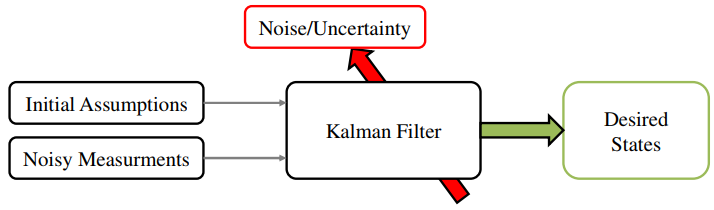
\includegraphics[width=\textwidth]{Chapters/Fig/kalman_dig.png}
        \caption{Diagram of Kalman filter}
        \label{fig:kalman_dig}
\end{figure}\par
Diagram of Kalman filter in fig.\ref{fig:kalman_dig} shows the goal of the filter is to take in impefect information sort out the useful parts of interest, and to reduce the uncertainty or noise.\\
The Kalman filter model assumes that the state of a system that at a time $t$ derived from the prior state at the time $t-1$ defined by the following equation:
\begin{equation}
 \textbf{x}_t = \textbf{F}_t \textbf{x}_{t-1} + \textbf{B}_t \textbf{x}_t + \textbf{w}_t,
\end{equation}\par
where
\begin{itemize}
    \item $\textbf{x}_t$ is the current state vector containing the parameters of interest of the system (e.g, position, velocity, accelerant..) at time t
    \item $\textbf{u}_t$ is the vector containing control inputs
    \item $\textbf{F}_t$ is the state transition matrix which applies the effect of each system state parameters at time $t-1$ on the system state at time $t$
    \item $\textbf{B}_t$ is the control input which applies the effect of each control input parameter in the control input vector $\textbf{u}_t$ on the state vector
    \item $\textbf{w}_t$ is the vector containing the process noise terms fro each parameter in the state vector.
\end{itemize}

\hspace{0.5cm}Measurements of the system is defined as follow:
\begin{equation}
         \textbf{z}_t = \textbf{H}_t\textbf{x}_t + \textbf{v}_t,
\end{equation}

\hspace{0.5cm}where:
\begin{itemize}
    \item $\textbf{z}_t$ is the vector of measurements
    \item $\textbf{H}_t$ is the transformation matrix that maps the state vector parameters into the measurement domain
    \item $\textbf{v}_t$ is the vector containing the measurement noise terms for each observation in the measurement vector
\end{itemize}\par
There is no direct observation of the true state $\textbf{x}_t$ of the system, and the Kalman filter provides an algorithm to estimate $\hat{\textbf{x}}_t$ using combination of models the system and noisy measurements. Hence, for now, the terms in interest in the state vector are distributed by Gaussian probability density functions (pdfs) rather than discrete values. Gaussian pdfs come up a co-variance matrix $\textbf{P}_t$ which has the diagonal containing the variances associated with the corresponding terms in the state vector and the remaining containing the co-variance between terms in the state vectors.\\
In the prediction state, initial state estimate, $\hat{\textbf{x}}_0$ and $\textbf{P}_0$ are applied recursively at each time step, using a loop then the current state vector is predicted from the state dynamic equation defined as:
\begin{center}
    $
        \hat{\textbf{x}}_{k|k-1} = \textbf{F}_{k-1}\hat{\textbf{x}}_{k-1} + \textbf{G}_{k-1}\textbf{u}_{k-1}, 
    $
\end{center}
\hspace{0.5cm}where:
\begin{itemize}
    \item $\hat{\textbf{x}}_{k|k-1}$ is the predicted state vector
    \item $\hat{\textbf{x}}_{k}$ is the previous estimated state vector
    \item $\textbf{u}$ is the input vector
    \item $\textbf{F}$ and $\textbf{G}$ are the matrices defining the system dynamics
\end{itemize}

\hspace{0.5cm}Then we predict the state error co-variance matrix by following:
\begin{equation}
          \textbf{P}_{k|k-1} = \textbf{F}_{k-1}\textbf{P}_{k-1}\textbf{F}^T_{k-1} + \textbf{Q}_{k-1}, 
\end{equation}

where:
\begin{itemize}
    \item $\textbf{P}_{k|k-1}$ is the predicted state error co-variance matrix
    \item $\textbf{P}_{k-1}$ is the previous estimated state error co-variance matrix
    \item $\textbf{Q}$ is the process noise co-variance matrix.
\end{itemize}\par
One the predicted valued are obtained, the Kalman gain matrix, $\textbf{K}_k$ is calculated by the following function:
\begin{equation}
              \textbf{K}_k = \textbf{P}_{k|k-1} \textbf{H}^T_k(\textbf{H}_k\textbf{P}_{k|k-1} \textbf{H}^T_k + \textbf{R}_k)^{-1},  
\end{equation}

with $\textbf{R}$ is the measurement noise co-variance.\par
The measurement update equations:
\begin{itemize}
    \item The state vector is updated as:
        \begin{equation}
                      \hat{\textbf{x}}_k = \hat{\textbf{x}}_{k|k-1} + \textbf{K}_k(\textbf{z}_k - \textbf{H}_x\hat{\textbf{x}}_{k|k-1}), 
        \end{equation}
    \item The state error co-variance is updated by
        \begin{equation}
                      \textbf{P}_k = (\textbf{I} -  \textbf{K}_k\textbf{H}_k)\textbf{P}_{k|k-1}, 
        \end{equation}
\end{itemize}
\pagebreak
\hspace{0.5cm}The workflow of Kalman filter is described in this the figure below:
\begin{figure}[h!]
    \centering
    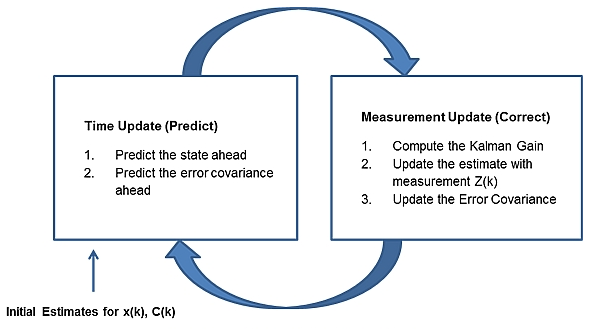
\includegraphics[scale=0.7]{Chapters/Fig/kal_dig_2.png}
    \caption{Workflow of Kalman filter}
    \label{fig:kalman_wf}
\end{figure}
\par
In fig.\ref{fig:kalman_wf}, two states "Predict" and "Correct" of Kalman filter occur continuously with the output of system in the time $t$ is the input of system in the time $t+1$, except the initial time $t_0$. The efficient recursive functions minimize the mean of the squared error in order to provide an optimal status of the model. In several respects, the filter is very powerful: it supports estimates of past, present, and even future states, and it can do so even if the model system's precise nature is unknown.






\section{Object Detection}
\hspace{0.5cm}Object detection is one of the essential tasks in computer vision, the aim of object detection is that localize the instances and classify them in a
image. With the outburst of deep learning for decades, deep learning based approaches have not only achieved state-of-the-art performance but also
solved the problem in real time speed.In this section, we would like describe two prominent algorithms in object detections.
\subsection{Faster Region Convolutional Neural Network}
\hspace{0.5cm}Faster R-CNN is the third version of Region Convolutional Neural Network (RCNN) family with some
improvements to increase the accuracy and the computational time. Instead of selective search to propose object region
for in two previous version R-CNN and Fast R-CNN, in Faster R-CNN, \cite{FrRCNN} proposed a network called \textit{Region Proposal Network} (RPN). The comparison of three versions in RCNN
family is shown in the fig.\ref{fig:rcnn_family}
\begin{figure}[h!]
    \centering
    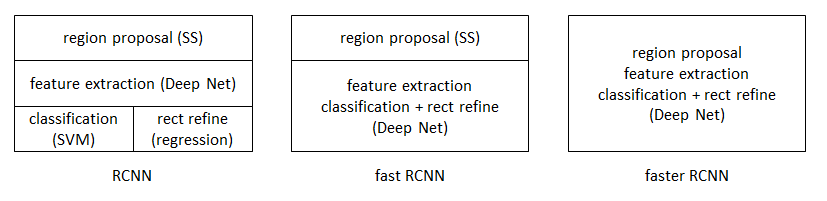
\includegraphics[width=\textwidth]{Chapters/Fig/rcnn-family.png}
    \caption{RCNN object detection frameworks}
    \label{fig:rcnn_family}
\end{figure}
\subsubsection{The algorithm}
\begin{figure}[h!]
    \centering
    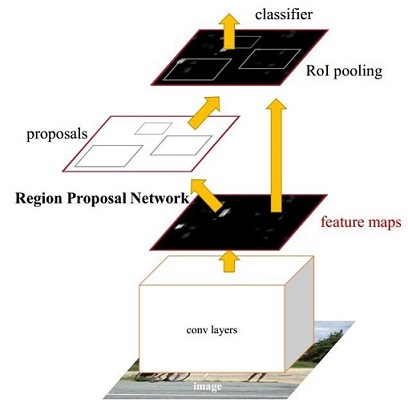
\includegraphics[width=0.5\textwidth]{Chapters/Fig/frrcnn.png}
    \caption{Faster RCNN workflow diagram}
    \label{fig:frrcnn_workflow}
\end{figure}
\hspace{0.5cm}First, the input picture is cropped and the cropped picture is going through a pre-trained classification network or feature extraction network (VGG, Inception, ResNet) to obtain feature map corresponding to the images.\par
Then, take 9 candidate regions of interest(ROIs) (3 different scales, 3 different aspect rations) on each anchor point on the feature map, and map them to the original image according to the corresponding scale.\par
Third, these candidate ROIs are then input into the RPN, which would determine whether these ROIs are foregroud or background and performs a preliminary regression (i.e. calculates the deviation of the bounding box between these foreground ROIs and the ground truth) and then do NMS\footnote{Non-maxima suppression}.\par
Next, perform ROI Pooling operations on these different sizes of ROIs (map the the ROIs to a specific size of feature map) and output a fixed size feature map.\par
Finally, it is input into a simple detection network, and then do classification and bounding box regression simultaneously.
\subsubsection{The architecture}
\begin{figure}[h!]
    \centering
    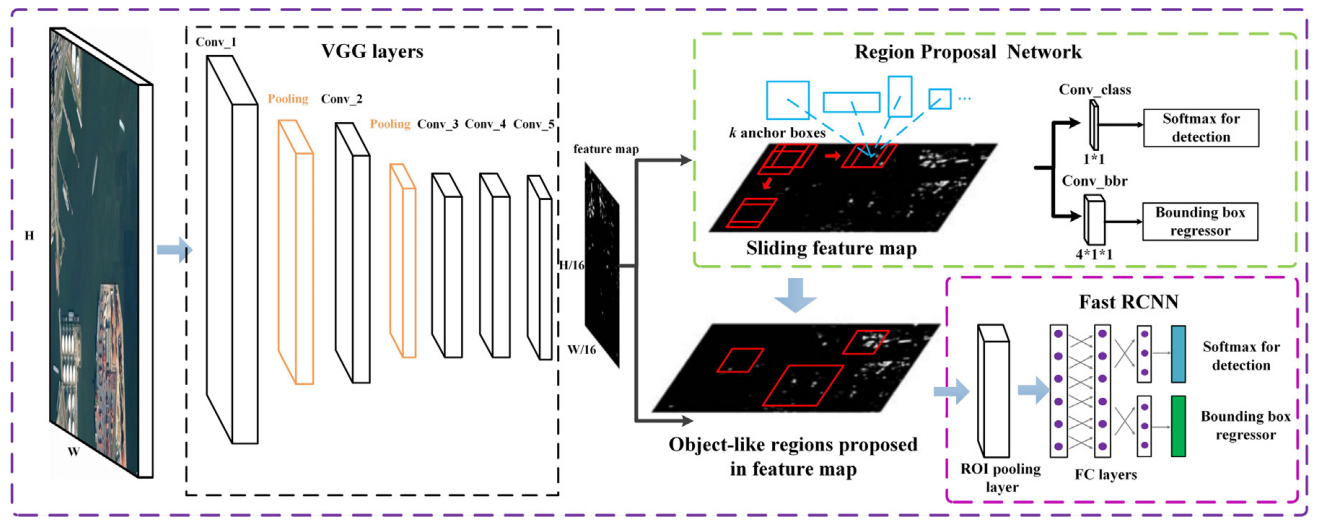
\includegraphics[width=0.8\textwidth]{Chapters/Fig/FrRCNN_arch.png}
    \caption{Faster RCNN architecture}
    \label{fig:frrcnn_arc}
\end{figure}
Faster RCNN adapts the architecture of two previous version of RCNN family and improve the computation time by using Region Proposal Network instead of using selective search in order to choose ROIs. In other words, Faster RCNN can be called RPN + Fast RCNN. For the feature extractor module. Faster RCNN using VGG16 pretrained on Image Net dataset.\par
The Region Proposal Network (RPN) visualized in fig.\ref{fig:RPN} is efficiently to propose ROIs of object in the image. RPN has a classifier and a regressor. Classifier determines the probability of a proposal having the target object. Regression regresses the coordinates of the proposals
\begin{figure}[h!]
    \centering
    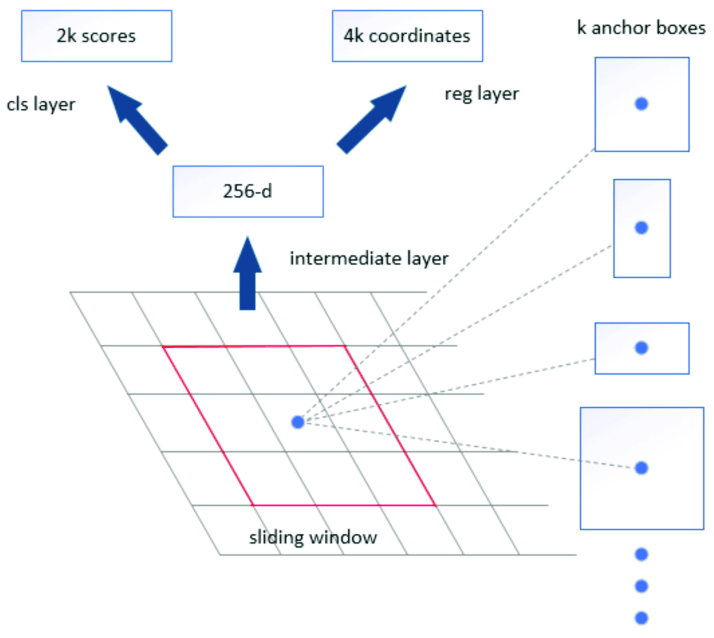
\includegraphics[width=0.6\textwidth]{Chapters/Fig/RPN_arc_1.png}
    \caption{Region Proposal Network mapping process}
    \label{fig:RPN}
\end{figure}
\par
It is a type of pooling layer which performs max pooling on inputs (here, convnet feature maps) of non-uniform sizes and produces a small feature map of fixed size (say 7x7). The choice of this fixed size is a network hyper-parameter and is predefined.The main purpose of doing such a pooling is to speed up the training and test time and also to train the whole system from end-to-end (in a joint manner).

\subsection{YOLOv3}
\hspace{0.5cm}YOLOv3 is the third version of object detection algorithm in YOLO (You Only Look One) family. It increase the accuracy and improve the performance with many modifications than the previous version and is more ability of detecting small objects.\par
\subsubsection{The algorithm}
\begin{figure}[h!]
    \centering
    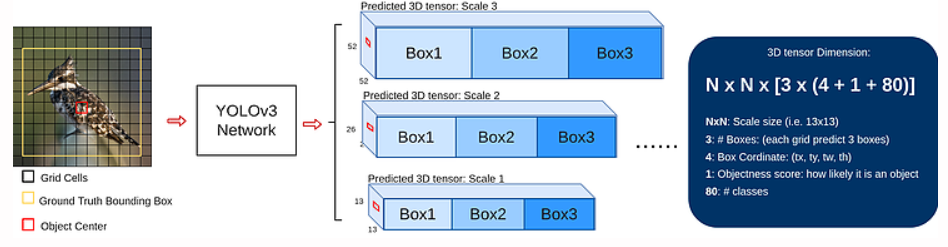
\includegraphics[width=\textwidth]{Chapters/Fig/yolo_algo.png}
    \caption{YOLOv3 Process Flow}
    \label{fig:1}
\end{figure}
\par
Firstly, YOLOv3 network predicts a 3D tensors with input images. The three scales processing is designed for detecting objects with various size in the input images. For example, with a scale of 13x13, the input image is divided into 13x13 grid cells and each grid cell corresponds to a 1x1x255 voxel inside the output 3D tensor. Concretely, 255 comes from (3 (anchor box/grid cell) x 4 (coordinates of predicted box) + 1 (object score) + 80 (class scores)).\par
Secondly, if the center point of the bounding box falls in a grid cell, this grid cell is responsible for evaluating the predicted bounding box of the object. For each grid cell, there are 3 anchor boxes assigned to it. The coordinates in the output tensor is the off-set values $t_x, t_y, t_w, t_h$, the applies the sigma function to constraint the offset values in range $[0,1]$. It makes the parametrization be easier to learn and the model is more stable\cite{Redmon_2017_CVPR}. \par In the fig.\ref{fig:bounding_box}, $(c_x, c_y)$ is the offset from the top left corner of the image grid, $(p_x, p_h)$ is the predefined width and height of the corresponding anchor box, while $b_x,b_y,b_w,b_h$ is the respect to the normalized coordinates of the center and the size of the predicted box.
The predicted box which has the highest objectness score, and IOU over the ground truth bounding box of the specfic class object is chosen.
\begin{figure}[h!]
    \centering
    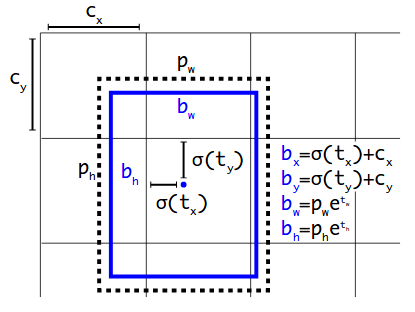
\includegraphics[scale=0.5]{Chapters/Fig/yolo_bounding_box.png}
    \caption{Predicted bounding box with dimensions priors and location prediction}
    \label{fig:bounding_box}
\end{figure}
\par
To choose the anchor boxes, the author uses the K-mean clustering algorithm to get 3 cluster means for each scale. this results in 9 sizes chosen from 9 clusters, 3 for 3 different scale.
\subsubsection{The architecture}
\begin{figure}[h!]
    \centering
    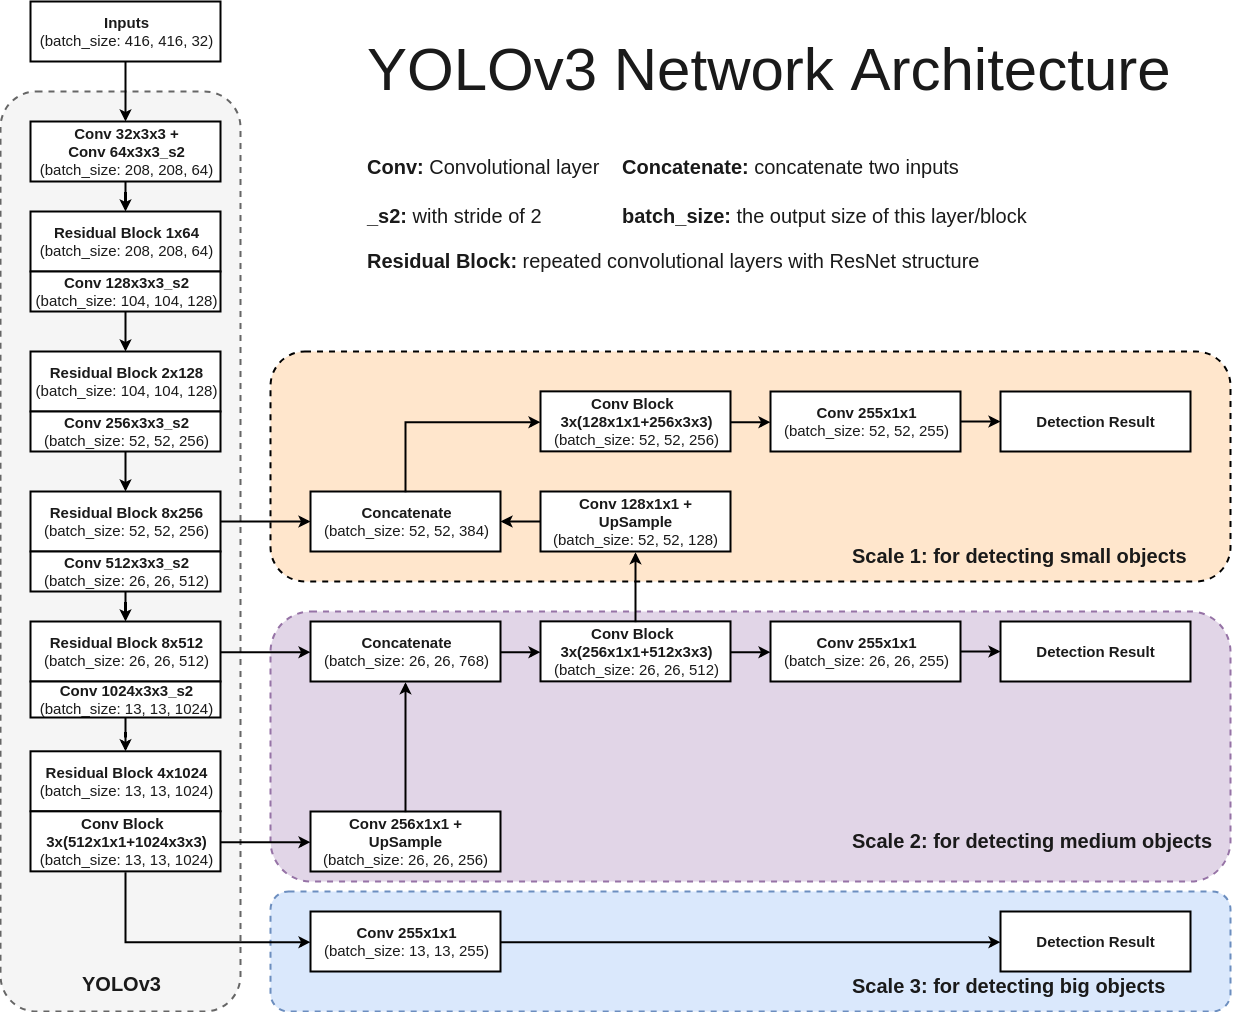
\includegraphics[scale=0.3]{Chapters/Fig/YOLOv3_architecture.png}
    \caption{YOLOv3 Network Architecture}
    \label{fig:yolo_arc}
\end{figure}
\par
 It is a feature-learning based network that adopts 75 convolutional layers as its most powerful
 tool. No fully-connected layer is used. This structure makes it possible to deal with images with
 any sizes. Also, no pooling layers are used. Instead, a convolutional layer with stride 2 is used
 to down-sample the feature map, passing size-invariant feature forwardly.  In addition, a
 ResNet-alike structure (residual blocks) and FPN-alike (Feature Pyramid Network) structure is also
 a key to its accuracy improvement. \par There is no \textit{softmax} layer in YOLOv3, it is
 replaced by a 1x1 convolutional layer with logistic regression. By using softmax, we have to
 assume that classes in the dataset are mutual independent while in some dataset, the labels are
 semantically similar. Training with softmax might not let the network generalize the data
 distribution well. Instead, a logistic function is used to deal with multi-label classification.

\section{Person Re-Identification}
\hspace{0.5cm}Person Re-identification is a task of detecting and precisely identifying a person from the a sequence images taken from different cameras or the same camera in different occasions. In this section, we would like to describe a creative approaches to solve this problem.
\subsection{Parameter-free Spatial Network for Person Re-Identification}

\subsubsection{The architecture}
\hspace{0.5cm} Global Average Pooling (GAP) can focus on effective information for regression problems, but it may also cause some information to be lost\cite{SA}. Therefore, the author added spatial attention before the GAP to improve the problem, as showing in fig.\ref{fig:sa_gap}, where FCN represents the fully connected layer FC.\par
 \begin{figure}[h!]
     \centering
     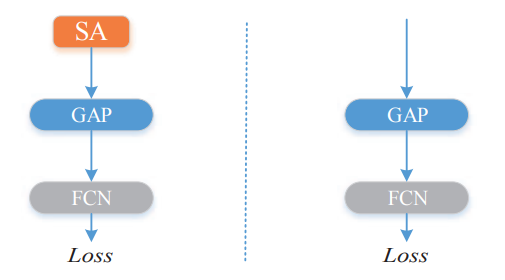
\includegraphics[scale=0.5]{Chapters/Fig/attention-sa-gap.PNG}
     \caption{Structure of a common classifier with GAP is shown on the right, the modification on the left is that a spatial attention layer (SA) is inserted before GAP}
     \label{fig:sa_gap}
 \end{figure}
The proposed network architecture is shown in fig.\ref{fig:sa_arc}.\par
\begin{figure}[h!]
    \centering
    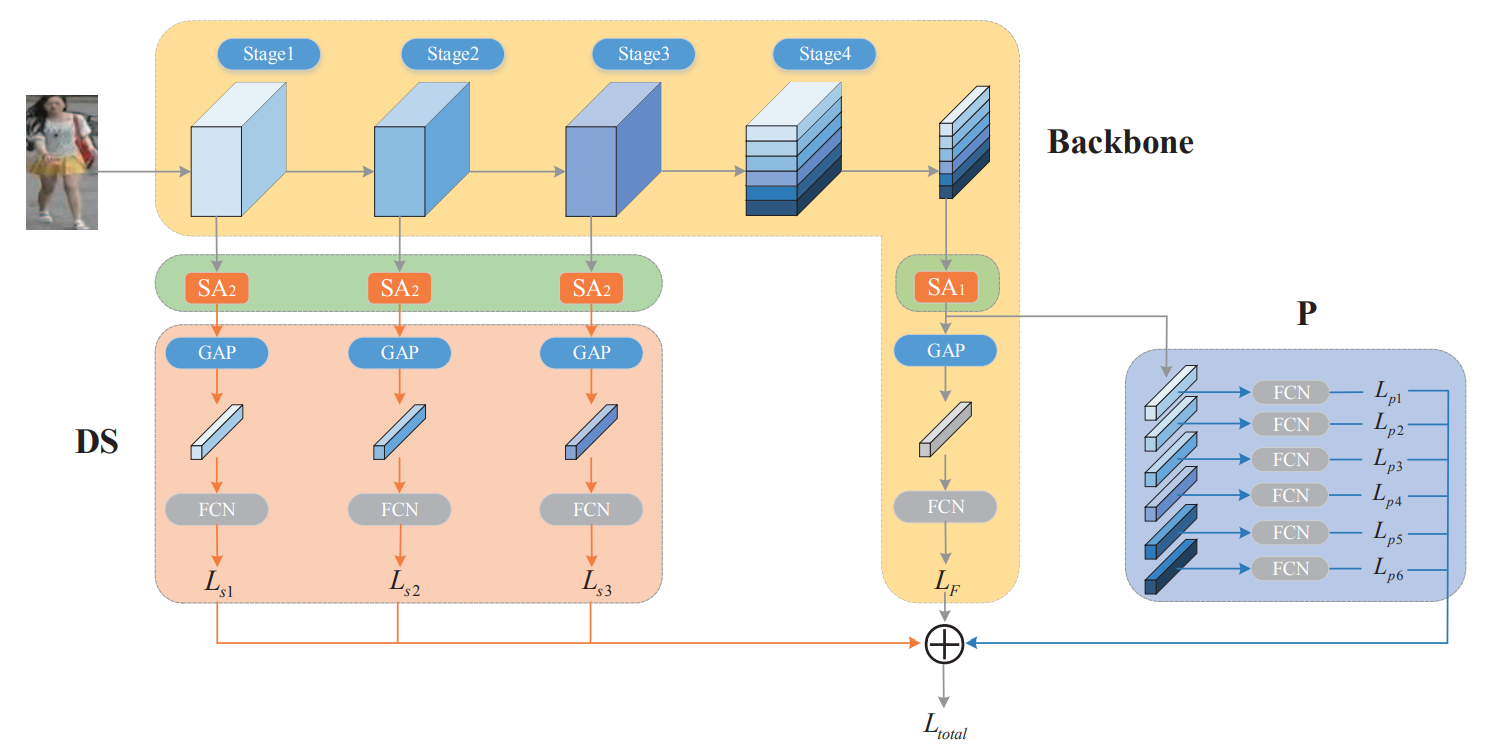
\includegraphics[width=0.6\textwidth]{Chapters/Fig/attention_network.PNG}
    \caption{The network architecture}
    \label{fig:sa_arc}
\end{figure}
The yellow part is the backbone ResNet-50. The red part represents the deep supervision branches, for which the spatial attention layers (the left green part) are added before GAP. The blue part denotes the part classifiers. Each part classifier produces a loss based on the part-level feature \cite{SA}. Note that the most right spatial attention part is not a part of the main model. It is only used in the ablation study \cite{SA}.\par
The input for every deeply supervised branch is a feature map $f$. The spatial attention layer first assigns different importance for different locations. The processed feature map is then fed into a GAP layer followed by a fully-connected layer before computing the cross-entropy loss $l_{si}$\cite{SA}. The losses calculated from three intermediate feature maps will in the end be added to the final loss\cite{SA}.\par
During testing, all the deeply supervised branches and
part classifiers on top are dismissed. The backbone will then
be used as a feature extractor, which is applied to all the
query images and the images in gallery to obtain the features. Then a standard information retrieval is performed
based on the Euclidean distance between these features.
\subsubsection{Parameter-free Spatial Attention}
\hspace{0.5cm}As shown in fig.\ref{fig:sa}, it is quite simple to compress the feature on the channel and use the method of directly adding the values of each channel to obtain a $H$x$W$x$1$ feature map, the reshape into a vector with size of $H$x$W$, then forward the vector through a softmax layer to obtain the weight of each element in the vector. Finally, we reshape vector of the weight to a volume with size of $H$x$W$x$1$ and concat with the original feature map.

\begin{figure}[h!]
    \centering
    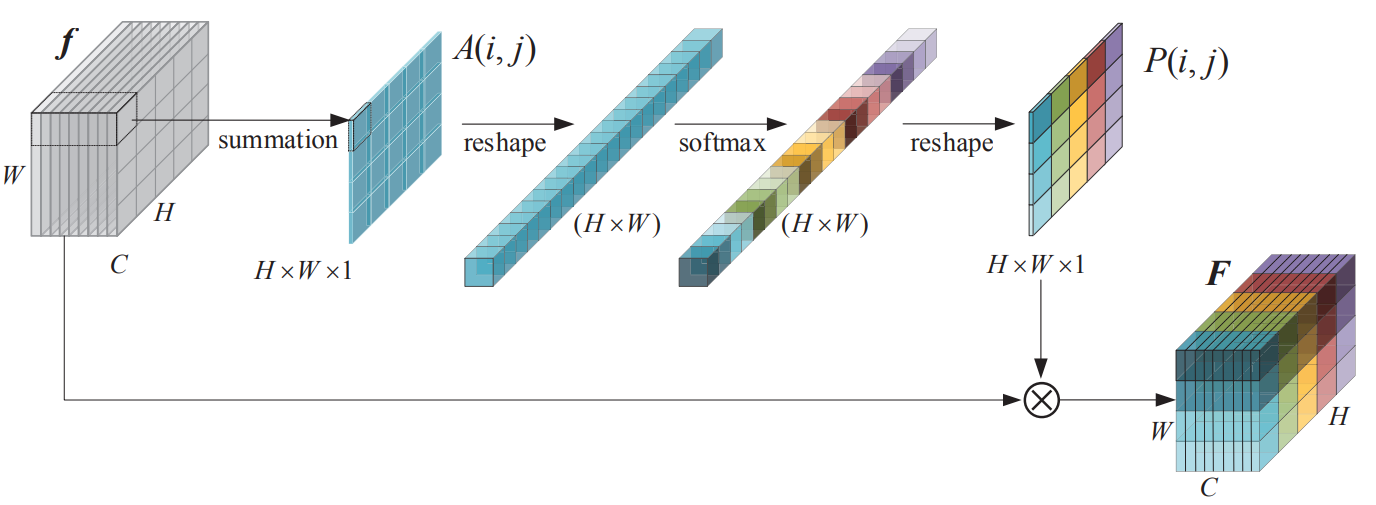
\includegraphics[scale=0.4]{Chapters/Fig/attention_sa.PNG}
    \caption{Parameter-free Spatial Attention Network Architecture}
    \label{fig:sa}
\end{figure}

\pagebreak
\section{Online pedestrian tracking methodologies}
\hspace{0.5cm} Online tracking-by-detection approaches usually operate the association the
detection of the current frame with a small number of the previous frames but not all the
information from the past. Otherwise, the performance of the method base on the detection quality,
it means occlusions or miss detections can produce fragment trajectories, assign wrong
identifications.However, there are now many advanced techniques proposed to overcome this
problem,for example, Yi et al. \cite{MultiTracking} introduced a method using two-stage association with affinity features
calculated from detections obtained by using ACF detector to address these problems. However, this approach
only uses the detections for tracking process and does not take the advanced of large-scale person re-identification datasets.
On the other hand, Wojke et al. \cite{Wojke2017simple} proposed DeepSORT, a method that takes both detections and predictions 
from trackers with multi-stage matching stages and uses the deep learning-based features to perform online pedestrian tracking.
In this section, we would like to discuss more about DeepSORT\cite{Wojke2017simple} which we determine to examine and propose some architecture alterations to this approach.\par

DeepSORT or Simple online and realtime tracking with a deep association metric \cite{Wojke2017simple} is 
the a improvement of SORT - Simple online and realtime tracking \cite{sort} . DeepSORT adapts effective parts from the previous version and integrates appearance information to improve the accuracy of SORT. All the computational complexity is placed 
into an offline pre-training stage where we learn a deep association metric on a large scale person re-identification dataset. \cite{Wojke2017simple}.
\subsection{Workflows}
\hspace{0.5cm} DeepSORT is a tracking-by-detection framework for the problem of multiple object tracking (MOT) where objects are detected in each frame and presented as bounding boxes \cite{sort}.\par
\begin{figure}[h!]
    \centering
    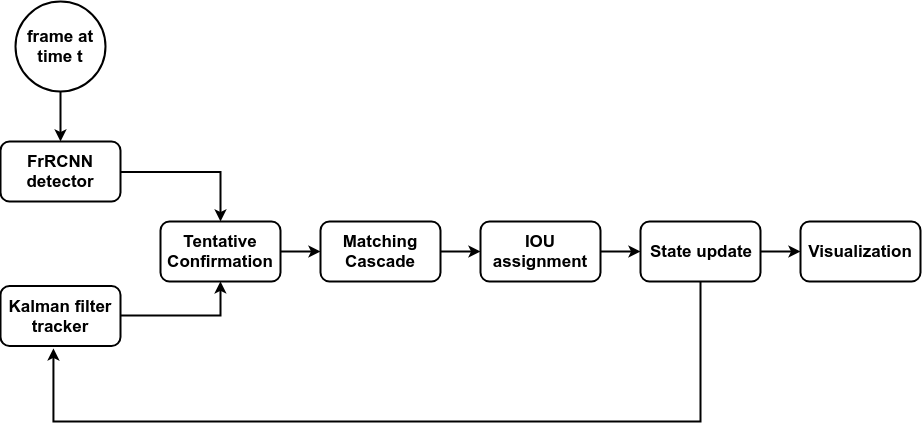
\includegraphics[width=\textwidth]{Chapters/Fig/Thesis_diagram-DeepSORT.png}
    \caption{DeepSORT workflow diagram}
    \label{fig:deepsort_workflow}
\end{figure}
In DeepSORT, for the tracking part, \cite{Wojke2017simple} uses Faster RCNN detector which has been pretrained on a collection of public and private datasets to provide excellent performance \cite{Wojke2017simple}, while in the tracking part, \cite{Wojke2017simple} uses a standard Kalman filter with constant velocity motion and linear observation model. The bounding coordinates $(u,v,\gamma,h)$ are taken as direct observations of the object state where $u,v$ is the bounding box center, $\gamma$ is the aspect ratio and $h$ is the height.\par
The results of tracking and detecting go through a tentative confirmation, then forward to two matching gates; 
firstly, \textit{Matching cascade}, workflow diagram of which shown in fig.\ref{fig:org_matching_cascade},
 secondly, \textit{IoU assignment} workflow diagram of which shown in fig.\ref{fig:org_iou}\par.
\begin{figure}[h!]
    \centering
    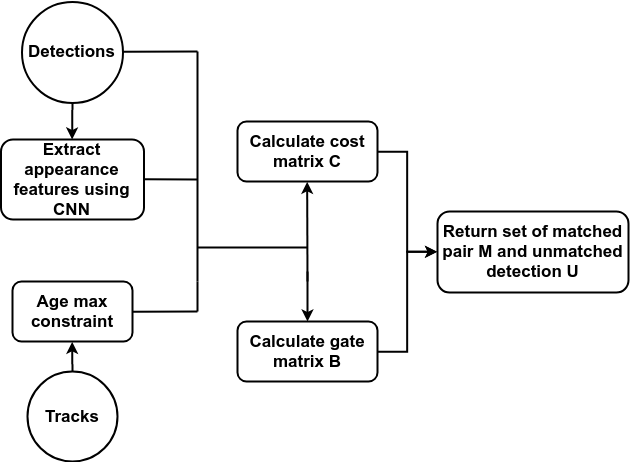
\includegraphics[width=0.8\textwidth]{Chapters/Fig/Thesis_diagram-CNN_Matching_Cascade.png}
    \caption{DeepSORT matching cascade}
    \label{fig:org_matching_cascade}
\end{figure}
\begin{figure}[h!]
    \centering
    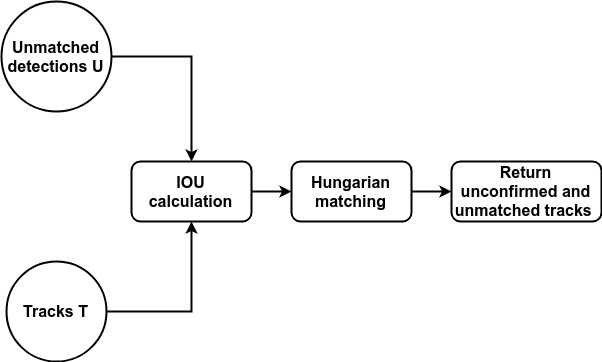
\includegraphics[width=0.8\textwidth]{Chapters/Fig/Thesis_diagram-IOU.png}
    \caption{DeepSORT IoU assignment}
    \label{fig:org_iou}
\end{figure}

\pagebreak
\cite{Wojke2017simple} define some constraints to match and suppress the detections and tracks:
\begin{itemize}
    \item For each track $k$, a number $a_k$ is the number of frames since the last successful measurement. This counter is incremented during Kalman filter prediction and assign to be zero when the track is associated with a measurement.
    \item Tracks that exceed a predefined maximum age $A_{max}$ are considered being deleted from the track set.
    \item New track hypotheses are initiated for each detection that cannot be associated to an existing track.
    \item New tracks are classified as tentative during their first three frames, during first three frames, a successful measurement association at each time step, if not, the track will be deleted.
\end{itemize}
\subsection{Motion information measurement}
\hspace{0.5cm} \cite{Wojke2017simple} proposed to use the Mahalanobis distance between predicted Kalman states and the newly arrived measurement
\begin{equation}
    d^{(1)}(i,j) = (d_j - y_i)^TS^-1_i(d_j-y_i)
\end{equation}
where $d_j$ indicates the position of the $j$-th detection box, $y_i$ indicates the predicted position of the $i$-th 
tracker to the target, $S_i$ indicates the co-variance matrix between the detected position and the average tracking position. \
The Mahalanobis distance takes into account the uncertainty of the state measurement by calculating the standard deviation between the detected position and the average tracking position.\par
If the Mahalanobis distance is less than a specified threshold $t^{(1)}$, the association is denoted by this binary indicator:
\begin{equation}
    b^{(1)}_{i,j}=\mathbb{1}[d^{(1)}(i,j) \leq t^{(1)}]
\end{equation}
$t^{(1)}$ is default set to 9.4877.\cite{Wojke2017simple}
\subsection{Appearance information measurement}
\hspace{0.5cm} Since the Mahalanobis distance provides only a rough estimate of object location, when motion uncertainty is high or occlusions occurs, motion information measurement is not enough. Hence, \cite{Wojke2017simple} proposed a second measurement using appearance features.\par
\begin{itemize}
    \item For each bounding box detection in $d_j$ aa appearance descriptor $r_j$ that is calculated from a  CNN model, 
    the architecture of which is shown on tab.\ref{tab:cnn_deepsort_arch} pre-trained on a large-scale re-identification dataset Market1501
    
    \item For a track $k$, keep a gallery $\mathcal{R}_k$ that stores feature vector of detection results for the last 100 frames that each tracking target successfully associated with.
     Then calculate the cosine distance between the $i$-th track and $j$-th detection in the appearance space:
    \begin{equation}
        d^{(2)}(i,j) = min\{1 - r_j^Tr^{(i)}_k | r^{(i)}_k\in \mathcal{R}_i\}
    \end{equation}
    \item A binary variable to indicate if an association is admissible to this metric:
    \begin{equation}
        b^{(2)}_{i,j}=\mathbb{1}[d^{(2)}(i,j) \leq t^{(2)}]
    \end{equation}
    $t^{(2)}$ is obtained from a separate training set
\end{itemize}
\hspace{0.5cm}The Mahalanobis distance provides information about possible object locations based on motion that are particularly useful for short-term predictions. On the other hand, the cosine distance considers appearance information that are particularly useful for recover ids after long-term occlusion.\par
Two metrics are combined by a weighted sum:
\begin{equation}
    c_{i,j} = \lambda d^{(1)}(i,j) + (1-\lambda d^{(2)}(i,j))
\end{equation}

The association is admissible if it is within the gate regions of both metrics:
\begin{equation}
    b_{i,j}=\Pi^2_{m=1}b^{(m)}_{i,j}
\end{equation}\par
In practical, the hyperparameter $\lambda$ is set to 0. Only appearance information are used in the association cost term when the Mahalanobis is useful in disregarding infeasible assignments inferred by the Kalman filter.
\begin{table}[H]
\begin{center}
 \begin{tabular}{||c c c ||} 
 \hline
 Name & Patch size/Stride & Output size \\ [0.5ex] 
 \hline\hline
 Conv1 & 3x3/1 & 32x128x64  \\ 
 Conv2 & 3x3/1 & 32x128x64 \\
 Max Pool 3 & 3x3/2 & 32x64x32 \\
 Residual 4 & 3x3/1 & 32x64x32 \\
 Residual 5 & 3x3/1 & 32x64x32 \\
 Residual 6 & 3x3/1 & 64x32x16 \\
 Residual 7 & 3x3/1 & 64x32x16 \\
 Residual 8 & 3x3/1 & 128x16x8 \\
 Residual 9 & 3x3/1 & 128x16x8 \\
 Dense 10   &       & 128    \\
 Batch and $\mathnormal{l}_2$ normalization &  & 128 \\
 \hline

 \hline
\end{tabular}
\end{center}
    \caption{CNN architecture of deep feature extractor in DeepSORT}
    \label{tab:cnn_deepsort_arch}
\end{table}
\subsubsection{Matching Cascade}
\begin{algorithm}
\caption{Matching Cascade}\label{algo:ds_matching}
\begin{algorithmic}[1]
\INPUT Tracking indices $\mathcal{T} = \{1, .. N\}$, Detection indices $\mathcal{D} = \{1, .. M\}$, Maximum age $A_{max}$

\State Compute cost matrix $\mathbf{C} = [c_{i,j}]$ using in Eq 3.3
\State Compute gate matrix $\mathbf{B} = [b_{i,j}]$ using in Eq 3.4
\State Initialize set of matches $\mathcal{M} \leftarrow \emptyset$
\State Initialize set of unmatched detection $\mathcal{U}\leftarrow\mathcal{D}$
\For{$n \in \{1, .., A_{max}\}$}
\State Select tracks by age $\mathcal{T}_n \leftarrow \{i \in \mathcal{T} | a_i = n\}$
\State $[x_{i,j}]\leftarrow$ min\_cost\_matching($\mathbf{C}, \mathcal{T}_n, \mathcal{U})$
\State $\mathcal{M} \leftarrow \mathcal{M} \cup \{(i,j) | b_{i,j}\cdot x_{i,j} > 0 \}$
\State $\mathcal{U} \leftarrow \mathcal{U}$ /\ $\{j |\underset{i}{\sum}b_{i,j}\cdot x_{i,j} > 0 \}$
\EndFor
\State Return $\mathcal{M}, \mathcal{U}$
\end{algorithmic}
\end{algorithm}
When an object is occluded for a longer period of time and two tracks compete for the same
detection, the Mahalanobis distance favors uncertainty, because it effectively reduces the
distance in the standard deviation of any detection toward the projected
track mean which can lead to increase track fragmentation and unstable tracks.\cite{Wojke2017simple}
Wojke et al.\cite{Wojke2017simple} introduced a matching cascade shown in algo.\ref{algo:ds_matching}
that gives priority to more frequently seen objects.\par
The subset of tracks $\mathcal{T}_n$ that have not been associated in last $n$
frames is considered to estimate linear assignment between tracks in $\mathcal{T}_n$ and undetected
detection $\mathcal{U}$. The matching cascade algorithm return set of matches and unmatched
detection. Then, to the final stage, using IoU (intersection over union) with Hungarian
algorithms to associate unmatched and unconfirmed track at age $n=1$ and the unmatched detection. This helps to to account for sudden appearance changes, e.g., due to partial occlusion with static scene geometry, and to
increase robustness against erroneous initialization\cite{Wojke2017simple}.\par




\section{Evaluation Metrics in MOT challenge}
\hspace{0.5cm}There has been a large number of metrics for quantitative evaluation of multiple target tracking has been proposed, however, due to the dataset for tracking problem in this work, the metrics in \cite{Milan2016MOT16AB} would be used and introduced in this section.
\subsection{Tracker-to-target assignment}
There are two common essentials to quantifying the performance of a tracker. Firstly, to determine for each hypothesized output, whether it is a true positive (TP) that describes an actual (annotated) output or the output is a false positive (FP), the decision is made by based on a defined distance measure $d$ which will be discussed later \cite{Milan2016MOT16AB}. If a target is not matched to any hypothesized output, it will be called a false negative (FN). In the other words, FP denotes for number of false detections and FN denotes for number of missed detections\cite{sort}. A result can be determined to be good if it has as few FPs and FNs as possible \cite{Milan2016MOT16AB}. Then, to measure by the number of false alarm per frame (FAF) or false positive per image (FPPI) in the object detection literature.\par
During the tracking process, it may happen that there are multiple outputs which covers the same target. The second prerequisite is then to establish the correspondence between all the annotated and hypothesized objects under the constraint that a true object should be recovered at most once, and that on hypothesis cannot account for more than one target \cite{Milan2016MOT16AB}. For the following, \cite{Milan2016MOT16AB} assumes that each ground truth trajectory has one unique start and end point. If a target leaves the FOV (field-of-view) and then reappears, the target would be assigned a new ID. Therefore, the current metrics do not explicitly handle target re-identification \cite{Milan2016MOT16AB}. To be more accurate, if a ground truth object $i$ is matched to hypothesis $j$ at time $t-1$ and the distance between $i$ and $j$ at frame $t$ is under the threshold distance, the correspondence between $i$ and $j$ still remain even if there exists a hypothesis $k$ that is closer distance to ground truth $i$. An identity switch is counted if a ground truth target $i$ is matched to a track $j$ and the last known assignment was $k\neq j$ \cite{Milan2016MOT16AB}.\par
\begin{figure}[h!]
    \centering
    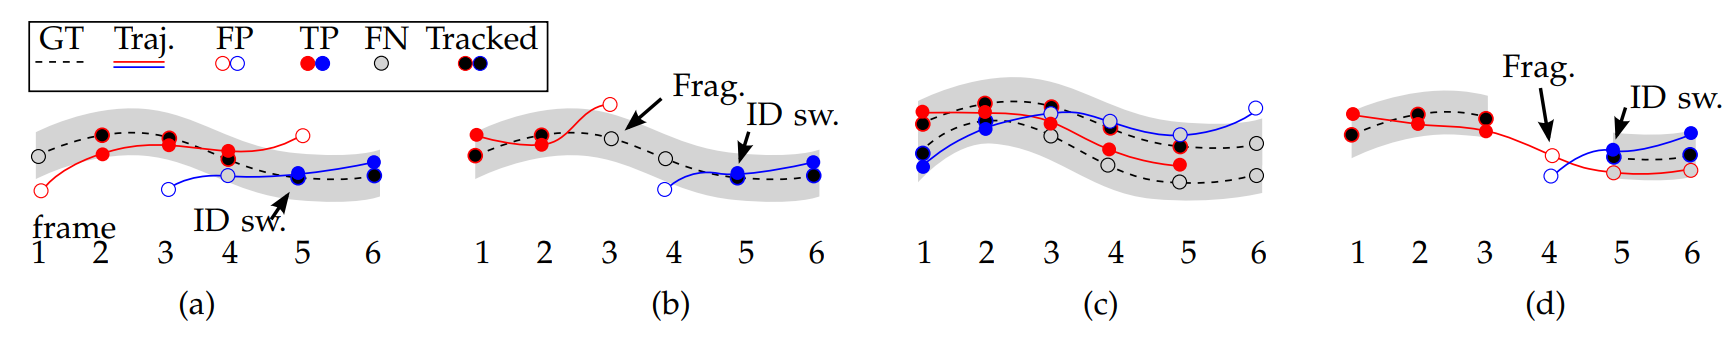
\includegraphics[width=0.8\textwidth]{Chapters/Fig/id_switch_mot.png}
    \caption{Four cases illustrating tracker-to-target assignments}
    \label{fig:ids_mot}
\end{figure}
Fig.\ref{fig:ids_mot} illustrated cases that cause ID switches in the tracking evaluation process. \cite{Milan2016MOT16AB} plots ground truth trajectories with dashed curved, and the tracker output with solid ones, where the color represents a unique target ID. The grey areas indicate the matching threshold (see next section). Each
true target that has been successfully recovered in one particular frame is represented with a filled black dot with a stroke color corresponding to its matched hypothesis.\par 
To be more detailed, (a) An ID switch occurs when the mapping switches from the previously assigned red track to the blue one. (b) A track fragmentation is counted in frame 3 because the target is tracked in frames 1-2, then interrupts, and then reacquires its ‘tracked’ status at a later point. A new (blue) track hypothesis also causes an ID switch at this point. (c) Although the tracking results are reasonably good, an optimal single-frame assignment in frame 1 is propagated through the sequence, causing 5 missed targets (FN) and 4 false positives (FP). Note that no fragmentations are counted in frames 3 and 6 because tracking of those targets is not resumed at a later point. (d) A degenerate case illustrating that target re-identification is not handled correctly. An interrupted ground truth trajectory will typically cause a fragmentation.
\subsection{Distance measure}
Because the presentation of objects in the image plane is the bounding box, to measure the similarity, \cite{Milan2016MOT16AB} employ intersection over union or IoU with the threshold $t_d$ is set to 0.5 or 50\%.
\subsection{Multiple Object Tracking Accuracy}
The multiple object tracking accuracy or MOTA is the most widely used metric to evaluate a tracker's performance because of its expressiveness as it combines three sources of the errors defined above:
\begin{equation}
    \text{MOTA} = 1 - \frac{\sum_t(\text{FN}_t + \text{FP}_t + \text{IDSW}_t)}{\sum_t\text{GT}_t}
\end{equation}
\subsection{Multiple Objects Tracking Precision}
Multiple objects tracking precision or MOTP is a measure of localization precision, not to be confused with positive predictive value or relevance in the context of precision/recall curves used in object detection\cite{Milan2016MOT16AB}. MOTP is the average dissimilarity between all true positives and their corresponding ground truth targets, the MOTP is defined as:
\begin{equation}
    \text{MOTP} = \frac{\sum_{t,i}d_{t,i}}{\sum_t c_t}
\end{equation}
where $c_t$ is the number of matches in frame $t$ and $d_{t,i}$ is the bounding box overlap of target $i$ with its assigned ground truth object.
\subsection{Tracking quality measures}
Each ground truth trajectory can be classified as mostly tracked (MT), partially tracked (PT), and mostly lost
(ML). This is done based on how much of the trajectory is recovered by the tracking algorithm. A target is mostly
tracked if it is successfully tracked for at least 80\% of its life span \cite{Milan2016MOT16AB}. If a track is only recovered for less than 20\% of its total length, it is said to be mostly lost (ML). All other
tracks are partially tracked. A higher number of MT and few ML is desirable.

